\documentclass[14pt]{article}
\usepackage{tikz}
%\usepackage[utf8]{vietnam}
\usetikzlibrary{shadings,calc}
\author{Lê Đình Mẫn\\ Email: ldman87@gmail.com}
\title{\textbf{Drawing in \LaTeX\ Using TikZ}}\date{}
\begin{document}
\maketitle\vskip-25pt\hrule\vskip10pt   
\begin{center}
    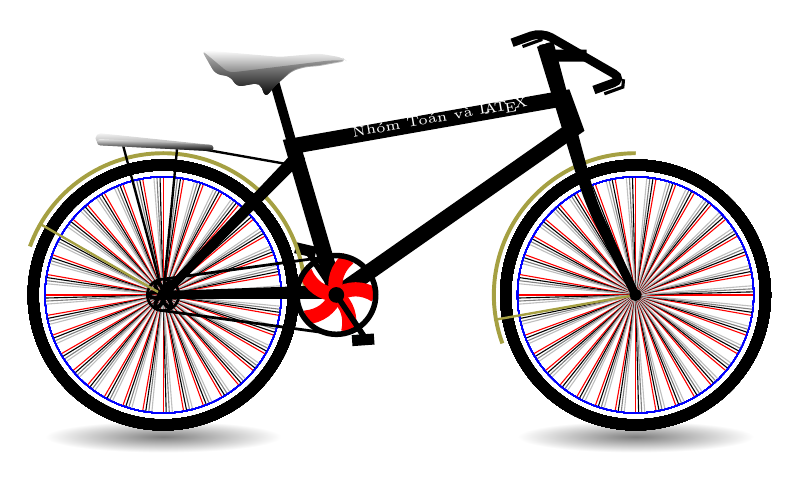
\begin{tikzpicture}[scale=1]
\shade[shading=radial] (-1.5,-2) rectangle (1.5,-1.6);
\shade[shading=radial] (4.5,-2) rectangle (7.5,-1.6);
\def\Radius{1.5cm}
\foreach \a in {0, 10, ..., 350} {  
    \draw[red] (0, 0) -- (\a:\Radius);
    \draw[black] (0, 0) -- (\a+1.5:\Radius);
    \draw[gray] (0, 0) -- (\a+3:\Radius);
    \draw[gray!50] (0, 0) -- (\a+4.5:\Radius);
    \draw[blue] (0, 0) circle[radius=\Radius];
    \draw[line width=4pt] (0, 0) circle[radius=\Radius+0.15cm];
}
\foreach \h in {0, 60, ..., 300} {
    \draw[color=black,line width=0.5mm,rotate around={\h:(0,0)}] (0,0) edge[-,bend left=40] (0.2cm,0) edge[-,bend right=40] (0.2cm,0);
}
\draw[line width=1pt] (0,0) circle[radius=0.2cm];
\draw[line width=4pt,rounded corners=1pt,rotate=0] (1.68,0.6)--(1.94,0.54);
\draw[line width=0.3mm,yellow!60!black] (1.8,0) arc (0:150:1.8cm)--(0,0);
\draw[line width=0.5mm,yellow!60!black] (1.8,0) arc (0:160:1.8cm);
\foreach \b in {0, 10, ..., 350} {  
    \draw[color=red,rotate around={\b:(6,0)}] (6, 0) -- (7.5,0);
    \draw[black,rotate around={\b+1.5:(6,0)}] (6, 0) -- (7.5,0);
    \draw[gray,rotate around={\b+3:(6,0)}] (6, 0) -- (7.5,0);
    \draw[gray!50,rotate around={\b+4.5:(6,0)}] (6, 0) -- (7.5,0);
    \draw[blue] (6, 0) circle[radius=\Radius];
    \draw[line width=4pt] (6, 0) circle[radius=\Radius+0.15cm];
}
\draw[line width=0.3mm,yellow!60!black] (6,1.8) arc (90:190:1.8cm)--(6,0);
\draw[line width=0.5mm,yellow!60!black] (6,1.8) arc (90:200:1.8cm);
\draw[line width=1pt] (0,0.2cm)--(2.2,0.5cm) (0,-0.2cm)--(2.2,-0.5cm);
\draw[line width=2pt] (2.2,0)--(2.6,-0.6) (2.2,0)--(1.8,0.6);
\draw[line width=1mm,rounded corners=8pt,rotate around={25:(6,0)}] (6,0)--(6,1.3cm)--++(80:2.1cm);
\draw[line width=1mm,rounded corners=8pt,rotate around={27:(6,0)}] (6,0)--(6,1.3cm)--++(80:2.1cm);
\draw[line width=1mm,rounded corners=8pt,rotate around={26:(6,0)}] (6,0)--(6,1.3cm)--++(80:2.1cm)coordinate(a);
\draw[line width=1.5mm] (a)--++(-80:0.15cm)--++(0:0.5cm)--++(180:0.05cm)coordinate(b);
\draw[line width=1.1mm,rounded corners=4pt] (b)--++(-30:0.6cm)coordinate(c)--++(-160:0.4cm) (b)--++(150:0.6cm)coordinate(d)--++(200:0.4cm);
\draw[line width=0.4mm,rounded corners=0pt] (c)--++(-95:0.1cm)--++(-160:0.25cm) (d)--++(-95:0.1cm)--++(200:0.25cm);
\draw[line width=2mm,rotate around={35:(2.2,0)}] (2.2,0)--++(3.7,0)--++(75:0.4cm)--++(155:3.5)coordinate(e)--(2.2,0);
\draw[line width=1mm] (0,0)--(2.2,0) (0,0)--(45:2.5cm) (0,0)--(46.5:2.5) (0,0)--(2:2.2);
\draw[line width=1.2mm] (e)--++(106:0.9cm)--++(-74:0.1cm)coordinate(d);
\foreach \c in {0, 72, ..., 288} {\draw[color=red,line width=1.8mm,rotate around={\c:(2.2,0)}] (2.2,0) edge[-,bend left=30] (2.69,0);}
\draw[line width=2pt] (2.2,0) circle[radius=0.5cm];
\fill (2.2,0) circle[radius=0.1cm];
\draw[line width=4pt,rounded corners=1pt,rotate=0] (2.4,-0.58)--(2.68,-0.56);
\draw[line width=2pt] (2.2,0)--(2.6,-0.6);
\shade[top color=white,bottom color=black,rounded corners=2pt,rotate around={10:(d)}] (d)--++(220:2mm)--++(100:2mm)--++(180:3mm)--++(110:1.5mm)--++(160:2mm)--++(110:3.5mm)coordinate(i)--++(-15:10mm)--++(-5:5mm)--++(-20:3mm)coordinate(j)--++(-50:0.7mm)--++(180:4mm)--++(170:1mm)--++(-175:2mm)--(d);
\shade[top color=gray!50,bottom color=black,rounded corners=2pt,rotate around={10:(d)}] (d)--++(220:2mm)--++(100:2mm)--++(180:3mm)--++(110:1.5mm)--++(160:2mm)--++(110:3.5mm)--++(-50:4.5mm)--++(-3:13mm)--++(-10:2mm)--++(180:4mm)--++(170:1mm)--++(-175:2mm)--(d);
\filldraw[black] (0,0)circle(2pt) (6,0)circle(2pt);
\draw[line width=0.3mm] (0,0)--++(105:2cm)--++(-2:0.7cm)coordinate(g)--+(-10:1.5cm) (g)--(0,0);
\shade[top color=gray!10!white,bottom color=gray] (-0.8cm,1.9cm)--++(-3:1.4cm) arc (-90:90: 0.4mm)--++(174:1.4cm) arc (90:270: 0.65mm);
\shade[top color=gray!20,bottom color=black] (-0.8cm,1.9cm)--++(-3:1.4cm) arc (-90:90: 0.4mm)--++(177:1.4cm) arc (90:270: 0.4mm);
\node[text=\fontsize{2pt}{0}\selectfont,color=white,rotate around={10:(3,2.72)}] at (3,2.72) {\tiny Nhóm Toán và \LaTeX};
\end{tikzpicture}
\end{center}
\end{document}